 
\documentclass[../main.tex]{subfiles}

\begin{document}

\begin{table}
\centering
\begin{tabular}{l|lll} 
 \toprule
 Measure & EliIE \cite{kang2017eliie} & Chia \cite{kury2020chia} & \textbf{LCT Corpus} \\
 \hline
    Disease domain & Alzheimer's Disease & All & \textbf{All} \\
    No. of Eligibility Descriptions & 230 & 1,000 & \textbf{1,006} \\
    No. of Annotations & 15,596 & 68,174 & \textbf{105,816} \\
    No. of Entity types & 8 & 15 & \textbf{50} \\
    No. of Relation types & 3 & 12 & \textbf{51} \\
    Mean Entities per doc. & - & 46 & \textbf{105} \\
    Mean Relations per doc. & - & 19 & \textbf{49} \\
 \hline
\end{tabular}
\caption{\textbf{Annotation statistics for EliIE, Chia, and LCT corpora.}}
\label{tbl_corpora_compare}
\end{table}
\subsection*{Eligibility Criteria and Database Queries}
\noindent The NLP tasks involved in transforming eligibility criteria into database queries include \textbf{named entity recognition} (NER) to tag meaningful spans of text as named entities, \textbf{relation extraction} to classify relations between named entities, \textbf{normalization} to map named entities to common coded representations (e.g., ICD-10), \textbf{negation detection} to detected negated statements (e.g., "not hypertensive") and so on. Gold standard corpora quality can thus directly affect performance and the validation of each of these tasks. In this article, we only focus on design and development of the LCT corpus. Figure \ref{fig_lct_text2sql} illustrates why corpora structure and integrity are important for the task of query generation, using examples of eligibility criteria annotated using the LCT annotation schema and corresponding hypothetical Structured Query Language (SQL) queries. In the first eligibility criterion, "preeclampsia" is explicitly named, and thus can be directly normalized to an International Classification of Diseases-Tenth Revision (ICD-10) or other coded representation. However, eligibility criteria involving non-specific drugs, conditions, procedures, contraindications, and so on are used frequently in clinical trials. In the second criterion in Figure \ref{fig_lct_text2sql}, "diseases" in "diseases that affect respiratory function" is non-specific, and must be reasoned upon in order to determine appropriate codes, such as asthma, chronic obstructive pulmonary disease (COPD), or emphysema.  Programmatically reasoning to generate queries in such cases would be challenging and often impossible if the underlying semantics were not captured appropriately. With this in mind, we developed the LCT annotation schema in order to enable reasoning and ease query generation for real-world clinical trials use. As the second example in Figure \ref{fig_lct_text2sql} shows, the LCT annotation captures the semantics of complex criteria, with changes to "respiratory function" annotated using a \textit{Stability[change]} entity and \textit{Stability} relation, and the cause, "diseases" annotated with a \textit{Caused-By} relation. During query generation, a hypothetical algorithm can thus use LCT entities and relations to first normalize the span "respiratory function", then reason that asthma, COPD, emphysema, and other conditions can affect respiratory function and thus the generated query should find patients with those diagnoses.

\begin{figure}[t]
  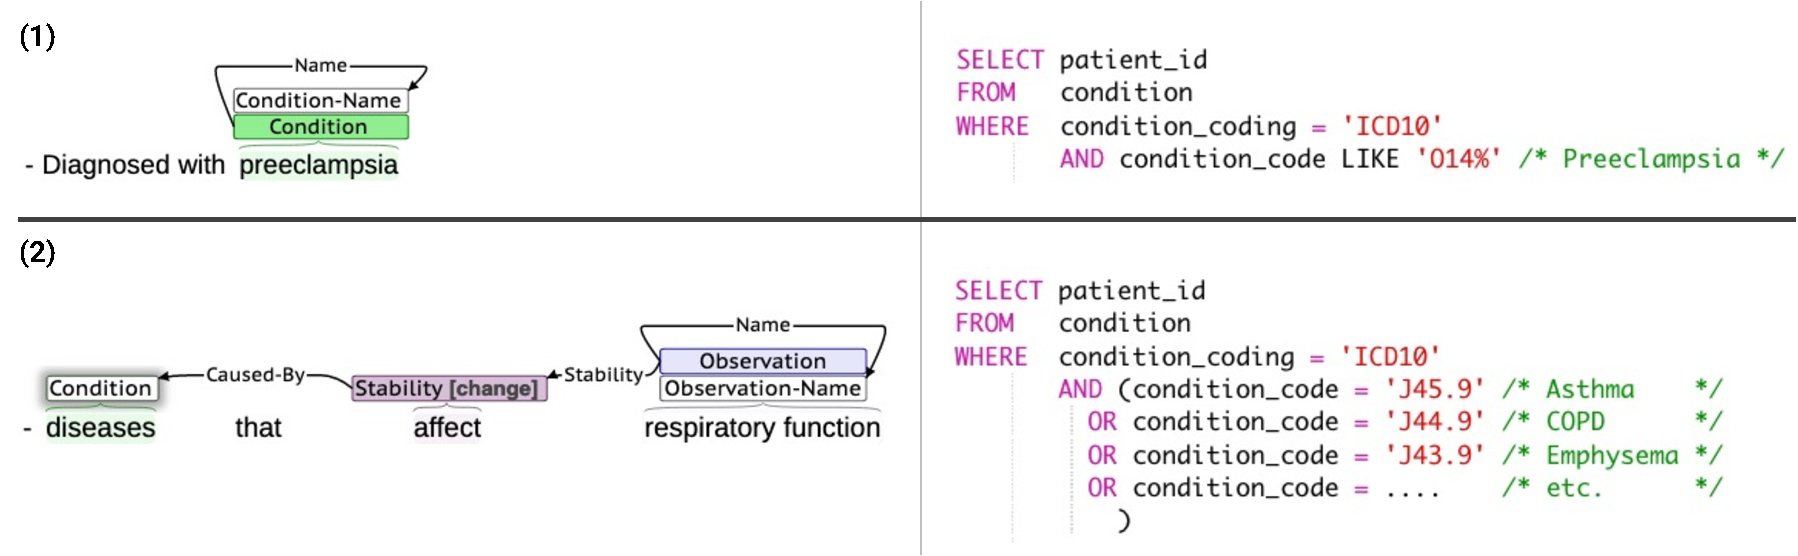
\includegraphics[scale=0.57]{figs/lct_text2sql.pdf}  
\caption{Example eligibility criteria annotated used the LCT corpus annotation schema (left) and corresponding example SQL queries (right) using a hypothetical database table and columns. Annotations were done using the Brat annotation tool \cite{stenetorp2012brat}. The ICD-10 codes shown are examples and not intended to be exhaustive.}
\label{fig_lct_text2sql}
\end{figure}

\subsection*{Annotation schema}

\noindent We aimed to develop an expressive, task-oriented annotation schema which could capture a wide range of medical concepts and logical constructs present in eligibility criteria. To accomplish this, we first analyzed previously published corpora \cite{weng2011elixr,boland2012elixrtime,kang2017eliie,kury2020chia} and expanded the list of included biomedical phenomena to fully capture the context and logic present in real clinical trials criteria. As one example, we introduced an entity called \textit{Contraindication} to reflect where use of a given treatment is inadvisable due to possible harm to the patient. \\

\noindent The LCT annotation schema is designed with the following goals and assumptions:

\begin{enumerate}
    \item The annotation schema should be \textbf{practical} and  \textbf{task-oriented} with a focus on facilitating ease of query generation. 
    \item A greater number of \textbf{more specific}, \textbf{less ambiguous} annotated phenomena should be favored over a smaller number of possibly ambiguous ones.
    \item Annotations should be \textbf{easily transformable} into composable, interconnected programmatic objects, trees, or node-edge graph representations.
    \item The annotation schema should \textbf{model eligibility criteria intent and semantics} as closely as possible in order to ensure generated queries can do the same.
\end{enumerate}

\noindent The LCT annotation schema is composed of \textbf{entities} and 
\textbf{relations}. Entities refer to biomedical, demographic, or other named entities relevant to eligibility criteria, and are annotated as a span of one or more tokens. We organized LCT entities into the following categories:
\begin{itemize}
    \item \textbf{Clinical} - \textit{Allergy, Condition, Condition-Type, Code, Contraindication, Drug, Encounter, Indication, Immunization, Observation, Organism, Specimen, Procedure, Provider}. %14
    \item \textbf{Demographic} - \textit{Age, Birth, Death, Ethnicity, Family-Member, Language, Life-Stage-And-Gender}. %21
    \item \textbf{Logical} - \textit{Exception, Negation}. %23
    \item \textbf{Qualifiers} - \textit{Acuteness, Assertion, Modifier, Polarity, Risk, Severity, Stability}. %30
    \item \textbf{Temporal and Comparative} - \textit{Criteria-Count, Eq-Comparison} (an abbreviation of "Equality Comparison"), \textit{Eq-Operator, Eq-Temporal-Period, Eq-Temporal-Recency, Eq-Temporal-Unit, Eq-Unit, Eq-Value}. %38
    \item \textbf{Other} - \textit{Coreference, Insurance, Location, Other, Study}. %43
\end{itemize}

\noindent The LCT corpus also includes 7 \textit{Name} entities: \textit{Allergy-Name}, \textit{Condition-Name}, \textit{Drug-Name}, \textit{Immunization-Name}, \textit{Observation-Name}, \textit{Organism-Name} and \textit{Procedure-Name}. \textit{Name} entities serve a special purpose in the LCT corpus, as they indicate that a span of text refers to a \textit{specific} condition, drug, etc., as opposed to \textit{any} condition or drug. \textit{Name} entities overlap with their respective general entities. For example, the span "preeclampsia" refers to a specific condition, and would thus be annotated as both a \textit{Condition} and \textit{Condition-Name}, while the span "diseases" is non-specific and would be annotated as only \textit{Condition}. A full listing of the LCT annotation guidelines can be found at \url{https://github.com/uw-bionlp/clinical-trials-gov-annotation/wiki}. \\

% 43 listed, plus 7 "-Name", 50 total
\noindent We defined a total of 50 entities in the LCT corpus. Examples of selected representative entities are presented in Table \ref{tbl_entity_examples}. In our representation, a subset of entities have \textbf{values} as well. For example, an \textit{Encounter} may have a value of \textit{emergency}, \textit{outpatient} or \textit{inpatient}. Values are optional in some entities (such as \textit{Encounters} or \textit{Family-Member}, where they may not always be clear or are intentionally broad) and always present in others. In the example annotations presented below, values are denoted using brackets ("[...]") following entity labels. \\

\begin{table}
    \def\arraystretch{1.3}
\begin{tabular}{m{2cm} m{2.5cm} m{4.9cm} m{6.5cm}}
    \toprule
    \textbf{Category} & \textbf{Entity} & \textbf{Values} & \textbf{Example Text}\\
    \hline 
    &
        Condition 
            & --  
            & Diagnosed with $\underset{Condition}{\underline{\mathrm{hypertension}}}$ in past year \\
     & Contraindication
            & --
            & any $\underset{Contraindication}{\underline{\mathrm{contraindications}}}$ to vaginal delivery \\
     & Drug 
            & -- 
            & on $\underset{Drug}{\underline{\mathrm{beta\ blockers}}}$ \\
     Clinical & Encounter 
            & emergency, outpatient, inpatient 
            & recently $\underset{Encounter[inpatient]}{\underline{\mathrm{admitted}}}$ to a hospital \\
     & Immunization 
            & --
            & received $\underset{Immunization}{\underline{\mathrm{Influenza\ vaccination}}}$ \\
     & Observation
            & lab, vital, clinical-score, survey, social-habit
            & $\underset{Observation[lab]}{\underline{\mathrm{Platelet\ count}}}$ less than 500 \\
     & Procedure
            & -- 
            & Undergoing or scheduled for a $\underset{Procedure}{\underline{\mathrm{colonoscopy}}}$ \\[2ex]
    \hline       
    \multirow{4}{}[-8pt]{\mbox{Demographic}} & 
        Age 
            & -- 
            & 43 years $\underset{Age}{\underline{\mathrm{old}}}$ \\
     & Birth
            & --
            & $\underset{Birth}{\underline{\mathrm{born}}}$ within the past 6 months \\
     & Family-Member 
            & mother, father, sibling, etc.
            & history of $\underset{Family-Member[mother]}{\underline{\mathrm{maternal}}}$ breast cancer \\
     & Language 
            & -- 
            & Speaks $\underset{Language}{\underline{\mathrm{English}}}$ or $\underset{Language}{\underline{\mathrm{Spanish}}}$  \\[2ex]
    \hline
    Logical &
       Negation 
            & -- 
            & with $\underset{Negation}{\underline{\mathrm{no}}}$ systemic disease \\
            
    \hline
    
    \multirow{6}{}[-16pt]{\mbox{Qualifier}} &
        Assertion
            & intention, hypothetical, possible
            & which $\underset{Assertion[hypothetical]}{\underline{\mathrm{may}}}$ cause conditions \\
         & Modifier
            & --
            & $\underset{Modifier}{\underline{\mathrm{alcohol}}}$ or $\underset{Modifier}{\underline{\mathrm{substance}}}$ abuse  \\
         & Polarity 
                & low, high, positive, negative 
                & showing $\underset{Polarity[high]}{\underline{\mathrm{elevated}}}$ serum creatinine  \\
         & Risk
            & -- 
            & at heightened $\underset{Risk}{\underline{\mathrm{potential}}}$ for suicide \\
         & Severity 
            & mild, moderate, severe 
            & with $\underset{Severity[severe]}{\underline{\mathrm{serious}}}$ complications from surgery  \\
         & Stability 
                & stable, change 
                & conditions known to $\underset{Stability[change]}{\underline{\mathrm{affect}}}$ mood \\[2ex]
    \hline
    \multirow{4}{}[-17pt]{\mbox{Temporal and} Comparative} &
        Criteria-Count
            & --
            & at least 3 of $\underset{Criteria-Count}{\underline{\mathrm{the\ following\ conditions}}}$: \\
     & Eq-Comparison
            & --
            & $\underset{Eq-Comparison}{\underline{\mathrm{greater\ than\ 50ml}}}$ \\
     
     & Eq-Temporal-Period
            & past, present, future
            & $\underset{Eq-Temporal-Period[present]}{\underline{\mathrm{Active}}}$ illness \\
     & Eq-Temporal-Recency
            & first-time, most-recent
            & $\underset{Eq-Temporal-Recency[most-recent]}{\underline{\mathrm{Latest}}}$ BMI > 35 \\
            
    \hline   
    Other &
       Location 
            & residence, clinic, hospital, unit, emergency-department  
            & Seen at $\underset{Location[clinic]}{\underline{\mathrm{diabetes\ care\ clinic}}}$ \\[2ex]
    
\end{tabular}

    \caption{\textbf{Examples of representative LCT annotation schema entities.} A full listing of all entities can be found in the LCT annotation guidelines at \url{https://github.com/uw-bionlp/clinical-trials-gov-annotation/wiki}.}
    \label{tbl_entity_examples}
\end{table} 

\noindent Relations serve as semantically meaningful connections between entities, such as when one entity acts upon, is found by, caused by, or related in some way to another. We categorize relations into the following:
\begin{itemize}
    \item \textbf{Alternatives and Examples} - \textit{Abbrev-Of, Equivalent-To, Example-Of}. %3
    \item \textbf{Clinical} - \textit{Code, Contraindicates, Indication-For, Name, Provider, Specimen, Stage, Type}. %10
    \item \textbf{Dependent} - \textit{Caused-By, Found-By, Treatment-For, Using}. %14
    \item \textbf{Logical} - \textit{And, If-Then, Negates, Or}. %18
    \item \textbf{Qualifier} - \textit{Acuteness, Asserted, Dose, Modifies, Polarity, Risk-For, Severity, Stability}.
    \item \textbf{Temporal and Comparative} - \textit{After, Before, Criteria, Duration, During, Max-Value, Min-Value, Minimum-Count, Numeric-Filter, Operator, Per, Temporal-Period, Temporal-Recency, Temporal-Unit, Temporality, Unit, Value}.
    \item \textbf{Other} - \textit{From, Except, Has, Is-Other, Location, Refers-To, Study-Of}.
\end{itemize}

\noindent We defined a total of 51 relations in the LCT corpus. Examples of relation criteria are shown in Table \ref{tbl_relation_examples}.  \\

\noindent In our annotations, some entity spans overlap with other entity spans in order to fully capture complex underlying semantics. Consider for example, the expression "Ages 18-55 years old". While an \textit{Age} entity may be assigned to token "Ages", if an \textit{Eq-Comparison} entity alone were assigned to the span "18-55 years old", the underlying semantics of the tokens "18", "-", "55", and "years" would be lost. In the following examples, we use the term \textbf{fine-grained entity} to refer to entities which are sub-spans of other \textbf{general entities}. Fine-grained entities are linked to general entities by relations. We use down arrow symbols (↓) to denote entity annotation and left and right arrow symbols (← and →) to denote relations. The (+) symbols denote overlapping entities on the same span. \\

\noindent The example expression "Ages 18-55 years old" would be annotated in three layers. In the first layer, the expression is annotated with \textit{Age} and \textit{Eq-Comparison} general entities with a relation between them: \\

\begin{center}
\begin{tabular}{c c c c c c c}
    "Ages" & & \multicolumn{5}{}{\underbrace{\text{"18 \, \, - \, \, 55 \, \, years \, \, old"}}} \\ 
    \big\downarrow & & \multicolumn{5}{c}{\big\downarrow}  \\
    \textit{Age} & \xrightarrow[Numeric-Filter]{} & \multicolumn{5}{c}{\textit{Eq-Comparison}} \\ \\
\end{tabular}
\end{center}
\\ \\

\noindent In the second layer, fine-grained entities with respective values are annotated: \\

\begin{center}
\begin{tabular}{c c c c}
    "18" & "-" & "55" & "years" \\ 
    \big\downarrow & \big\downarrow & \big\downarrow & \big\downarrow \\
    \textit{Eq-Value} & \textit{Eq-Operator} & \textit{Eq-Value} & \textit{Eq-Temporal-Unit} \\
     & \textit{[between]} & & \textit{[year]} \\
\end{tabular}
\end{center}

\noindent In the third layer, relations connecting fine-grained entities to the general \textit{Eq-Comparison} entity are added: \\

\begin{center}
\begin{tabular}{llll}
    \multirow{4}{5.5em}[-8pt]{\textit{\mbox{Eq-Comparison}}} & \multirow{4}{1em}[-4pt]{\begin{cases}\\\\\\\\\end{cases}} & \xrightarrow[Value]{} & \textit{Eq-Value "18"} \\
    & & \xrightarrow[Operator]{} & \textit{Eq-Operator[between]} "-" \\
    & & \xrightarrow[Value]{} & \textit{Eq-Value "55"} \\
    & & \xrightarrow[Temporal-Unit]{} & \textit{Eq-Temporal-Unit[year]} "years" \\
\end{tabular}
\end{center} \\

\noindent This multilayered annotation strategy allows significant flexibility in capturing entities and relations in a slot-filling fashion, simplifying the task of downstream query generation. We show examples of this in the Usage Notes section. \\

\begin{table*}[ht!]
    \centering
    \def\arraystretch{0.8}
\begin{tabular}{m{3.8cm} m{2.2cm} m{10cm}}
\toprule
    \textbf{Category} & \textbf{Relation} & \textbf{Example Annotation} \\ \midrule
    
     & Abbrev-Of     & $\underset{Condition}{\underline{\mathrm{Post\ Concussion\ Syndrome}}}$ \quad $\xleftarrow[Abbrev-Of]{}$ \quad ($\underset{Condition}{\underline{\mathrm{PCS}}}$) \\
        
    Alternatives and Examples & Equivalent-To & $\underset{Condition}{\underline{\mathrm{Thrombocytopenia}}}$ \quad $\xleftarrow[Equivalent-To]{}$ \quad $\underset{Observation[lab]}{\underline{\mathrm{platelets}}}$ \quad $>$ 100,000/mm3" \\
    
     & Example-Of    & $\underset{Condition}{\underline{\mathrm{skin\ condition}}}$ \quad $\xleftarrow[Example-Of]{}$ \quad (e.g. \quad $\underset{Condition}{\underline{\mathrm{eczema}}}$ )" \\[2ex] 
     
    \hline
     
     Clinical & Contraindicates & conditions \quad  $\underset{Contraindication}{\underline{\mathrm{contraindicating}}}$ \quad $\xrightarrow[Contraindicates]{}$ \quad $\underset{Procedure}{\underline{\mathrm{MRI}}}$ \\[2ex] 
    
    \hline
    
    \multirow{4}{*}[-13pt]{\mbox{Dependent}} &
        Caused-By     & $\underset{Observation}{\underline{\mathrm{swellings}}}$ \quad $\xrightarrow[Caused-By]{}$ \quad $\mathrm{due\ to}$ \quad $\underset{Condition}{\underline{\mathrm{trauma}}}$ \\    
        
     & Found-By      & $\underset{Observation}{\underline{\mathrm{lesion}}}$ \quad $\xrightarrow[Found-By]{}$ \quad $\mathrm{seen\ on\ standard}$ \quad $\underset{Procedure}{\underline{\mathrm{imaging}}}$ \\
    
     & Treatment-For & $\underset{Procedure}{\underline{\mathrm{coronary\ bypass\ surgery}}}$ \quad $\xrightarrow[Treatment-For]{}$ \quad $\mathrm{for}$ \quad $\underset{Condition}{\underline{\mathrm{atherosclerosis}}}$ \\
    
     & Using         & $\underset{Procedure}{\underline{\mathrm{total\ knee\ arthroplasty}}}$ \quad $\xrightarrow[Using]{}$ \quad $\mathrm{with}$ \quad  $\underset{Procedure}{\underline{\mathrm{spinal\ anesthesia}}}$ \\[2ex]
    
    \hline
    
    Logical &
        If-Then       & BMI \quad $\underset{Eq-Comparison}{\underline{\mathrm{greater\ than\ 38}}}$ \quad $\xleftarrow[If-Then]{}$ \quad $\mathrm{for}$ \quad $\underset{Life-Stage-And-Gender[female]}{\underline{\mathrm{women}}}$ \\[2ex]
         
    \hline
    
         & Risk-For & $\underset{Risk}{\underline{\mathrm{risk}}}$ \quad $\xrightarrow[Risk-For]{}$ \quad $\mathrm{of}$ \quad $\underset{Death}{\underline{\mathrm{death}}}$ \\
        Qualifier & Severity & $\underset{Severity[mild]}{\underline{\mathrm{mild}}}$ \quad $\xleftarrow[Severity]{}$ \quad $\underset{Observation}{\underline{\mathrm{symptoms}}}$ \\
         & Stability & $\underset{Observation}{\underline{\mathrm{hemodynamically}}}$ \quad $\xrightarrow[Stability]{}$ \quad $\underset{Stability[change]}{\underline{\mathrm{unstable}}}$ \\[2ex]
    
    \hline
    
     &
        After & $\underset{Condition}{\underline{\mathrm{infected}}}$ \quad $\xrightarrow[After]{}$ \quad $\mathrm{following}$ \quad $\underset{Encounter[inpatient]}{\underline{\mathrm{admission}}}$ \\
        
        & Before & $\mathrm{diagnosis of}$ $\underset{Condition}{\underline{\mathrm{aortic\ stenosis}}}$ \quad $\xrightarrow[Before]{}$ \quad $\mathrm{prior\ to}$ \quad $\underset{Encounter}{\underline{\mathrm{visit}}}$ \\
        
        & Duration & $\underset{Condition}{\underline{\mathrm{type\ 1\ diabetes}}}$ \quad $\xrightarrow[Duration]{}$ \quad $\mathrm{for}$ \quad $\underset{Eq-Comparison}{\underline{\mathrm{at\ least\ 1\ year}}}$ \\ 
        Temporal and Comparative & During & $\underset{Procedure}{\underline{\mathrm{mechanically \ ventilated}}}$ \quad $\xrightarrow[During]{}$ \quad $\mathrm{while}$ \quad $\underset{Encounter[inpatient]}{\underline{\mathrm{admitted}}}$ \\
        
         & Numeric-Filter & $\underset{Observation[vital]}{\underline{\mathrm{body\ weight}}}$ \quad $\xrightarrow[Numeric-Filter]{}$ \quad $\underset{Eq-Comparison}{\underline{\mathrm{less\ than\ 110\ pounds}}}$ \\    
        
         & Minimum-Count & $\underset{Encounter[inpatient]}{\underline{\mathrm{admitted}}}$ \quad $\xrightarrow[Minimum-Count]{}$ \quad $\underset{Eq-Comparison}{\underline{\mathrm{at\ least\ twice}}}$ \\    
        
         & Temporality & $\underset{Encounter}{\underline{\mathrm{seen}}}$ \quad $\xrightarrow[Temporality]{}$ \quad $\underset{Eq-Comparison}{\underline{\mathrm{within\ past\ 6\ months}}}$ \\[2ex]
         
    \hline
    
    Other &
         Location & $\underset{Encounter[inpatient]}{\underline{\mathrm{admitted}}}$ \quad $\xrightarrow[Location]{}$ \quad $\mathrm{to\ the}$ \quad $\underset{Location[unit]}{\underline{\mathrm{ICU}}}$ \\[2ex]
    
\end{tabular}
    \caption{\textbf{Examples of representative relations.} Direction of arrows indicates role, i.e., subject → target entity.}
    \label{tbl_relation_examples}
\end{table*}

\noindent The LCT annotation schema contributes the following novel features: (1) deep granularity in entities and relations, which enables (2) rich semantic representation, closely capturing the intent of complex clinical trial eligibility criteria and facilitating accurate query generation.

\subsubsection*{Deep Entity and Relation Granularity}
\noindent We assume that more specific annotation labels are generally more straightforward to generate accurate queries with. For example, within the span, "preceding six months", annotating the token "preceding" as \textit{Temporal} (an entity type in Chia) may appear to be adequate, given that an English-speaking human would understand that this refers to the past. Without further information, however, a naïve algorithm would be unable to determine (1) whether such a entity refers to the past, present, or future, (2) that the token "six" refers to a numeric value, and (3) that "months" refers to a unit of temporal measurement. In such cases, most query generation algorithms introduce additional rule-based or syntactic parsing modules, such as SuTime \cite{chang2012sutime} to further normalize the phrase to a value \cite{weng2011elixr, yuan2019criteria2query}. This ambiguity in label semantics creates unnecessary complexity in downstream systems, requiring that the same text be processed a second time. \\

\noindent In contrast, we designed the LCT annotation schema to favor discrete, explicit entities and relations where possible, with an aim toward reducing the need for additional normalization steps needed for query generation. In our annotation schema, this example would be annotated with the following fine-grained entities: \\

\begin{center}
\begin{tabular}{c c c}
    "preceding" & "six" & "months" \\ 
    \big\downarrow & \big\downarrow & \big\downarrow \\
    \textit{Eq-Temporal-Period} & \textit{Eq-Value} & \textit{Eq-Temporal-Unit} \\
    \textit{[past]} & & \textit{[month]} \\
\end{tabular}
\end{center}
\\ 
\noident As shown in the example, each token is uniquely annotated, with the values \textit{[past]} and \textit{[month]} serving to more clearly disambiguate semantics of the temporal phrase to a normalized temporal value. Moreover, as fine-grained entities are connected by relations to general entities, which can in turn have relations to other general entities, the LCT annotation schema is able to capture eligibility criteria semantics at a deeper level than other corpora. \\

\subsubsection*{Rich Semantic Representation}
\noindent Certain eligibility criteria cannot be directly translated into queries, but instead must first be reasoned upon. For example, a query to find patients meeting the criterion of "conditions contraindicating pioglitazone" requires reasoning to first answer the question, \textit{What} conditions contraindicate use of pioglitazone? Such reasoning may be performed by a knowledge base or other methods, but cannot be done unless the contraindicative relation is detected:

\begin{center}
\begin{tabular}{c c c c c}
    "Conditions" & & "contraindicating" & & "pioglitazone" \\ 
    \big\downarrow & & \big\downarrow & & \big\downarrow \\
    \textit{Condition} & \xleftarrow[Caused-By]{} & \textit{Contraindication} & \xrightarrow[Contraindicates]{} & \textit{Drug} \\[-1ex]
    & & & & + \\
    & & & & \textit{Drug-Name} \\
\end{tabular}
\end{center}

\noindent As the span "Conditions" is labeled \textit{Condition} but does not have an overlapping \textit{Condition-Name} entity, it is considered unnamed and thus would need to be reasoned upon to determine. "[P]ioglitazone", on the other hand, includes a \textit{Drug-Name} entity and is thus considered named. The absence of overlapping \textit{Name} entities serves as an indicator to downstream applications that reasoning may be needed to determine relevant conditions or drugs. We examine additional cases of the LCT's semantic representation and benefits in the next section, where we compare the LCT annotation schema to Chia's.

\begin{figure}[ht!]
  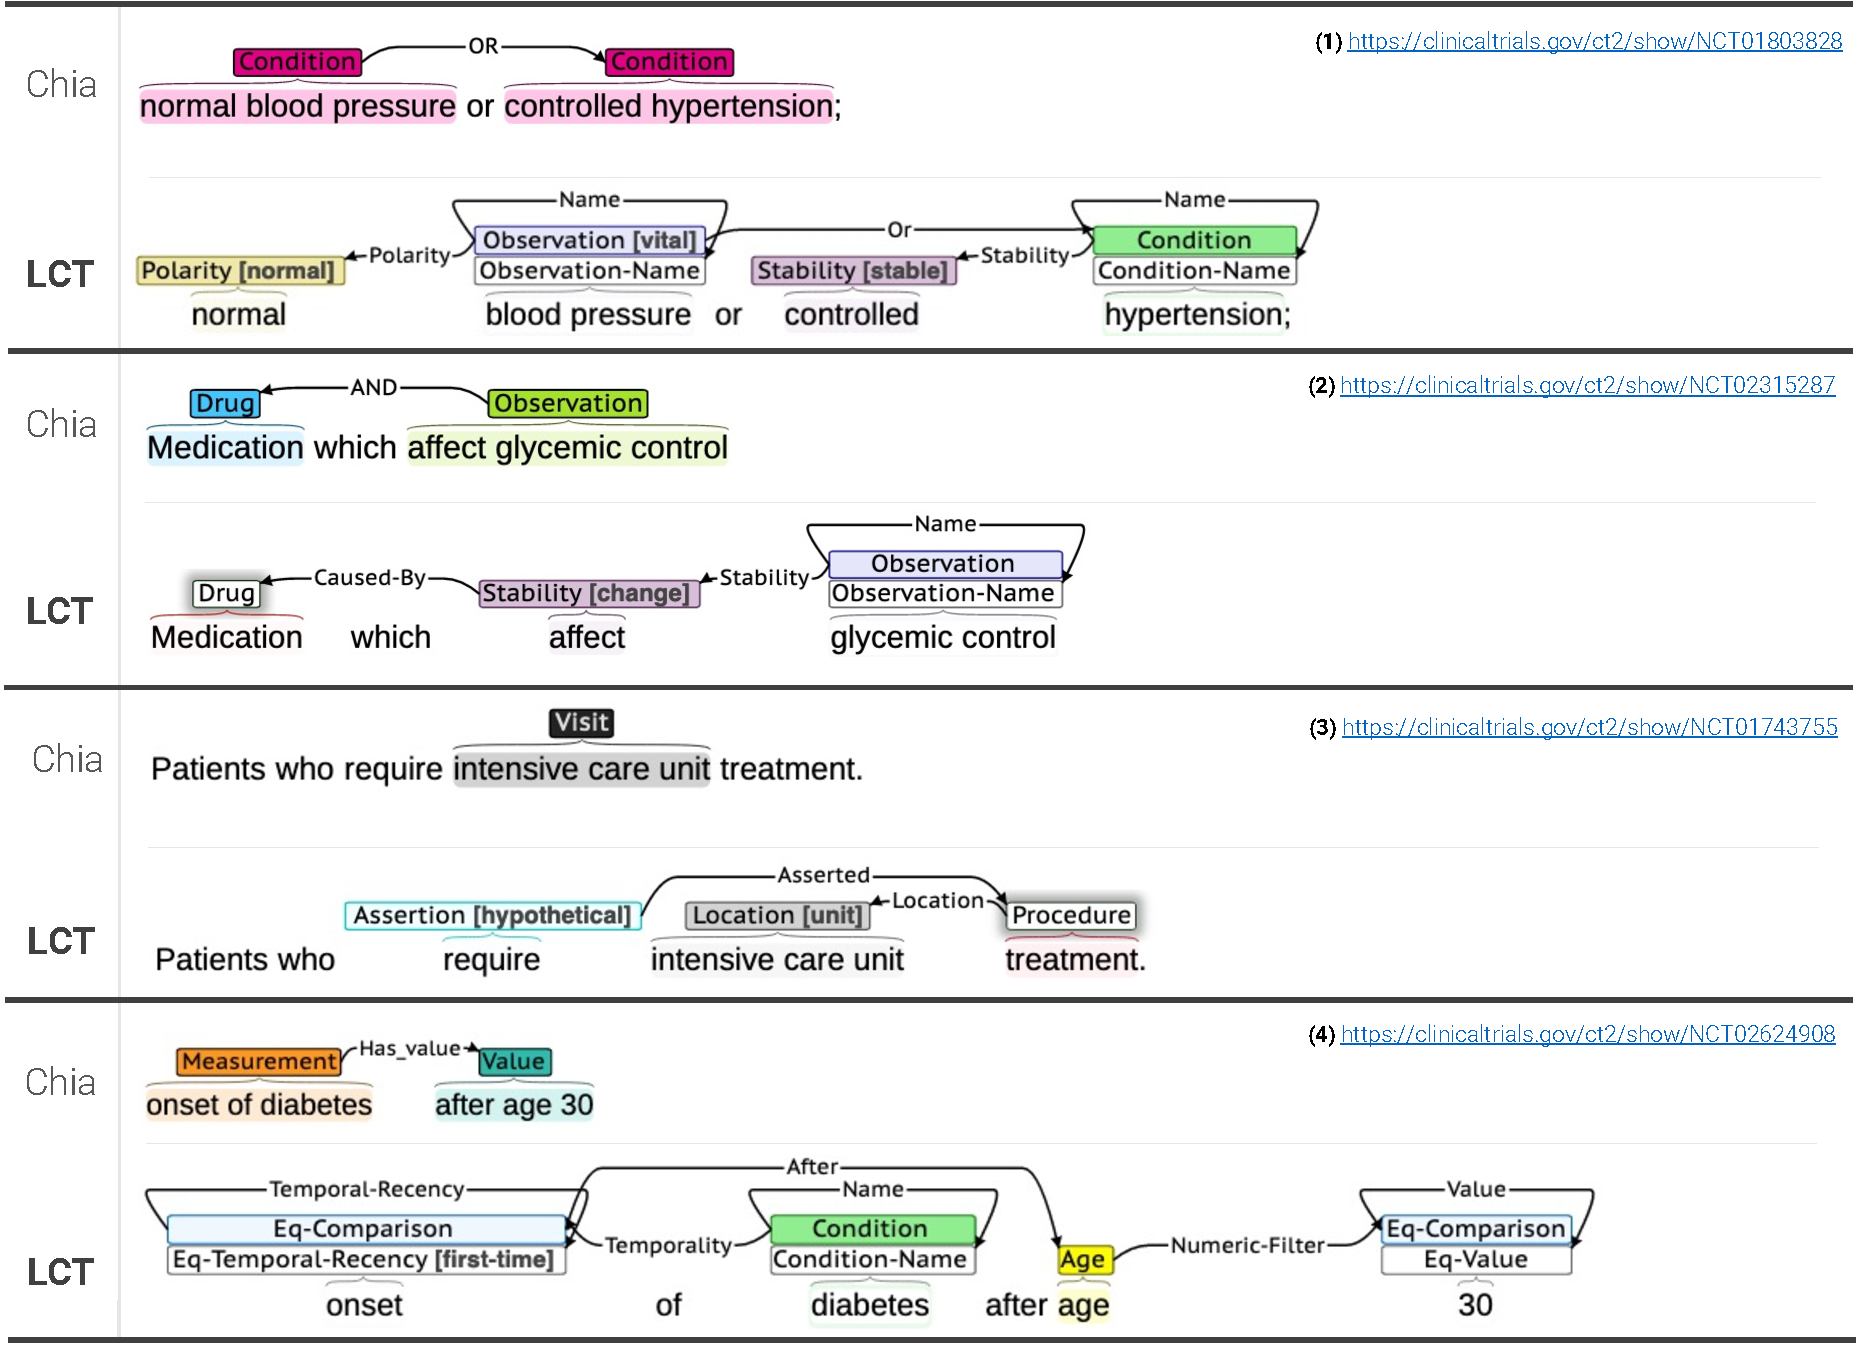
\includegraphics[scale=0.56]{figs/chia_vs_lct.pdf}  
    \caption{Examples of clinical trials eligibility criteria annotated with Chia and LCT annotation schemas. Each example shows a criterion from a Chia annotation (above) and an LCT annotation of the same text for purposes of comparison (below).}
    \label{fig_chia_vs_lct}
\end{figure}

\subsection*{Comparison to Chia}
We designed the LCT annotation schema by building upon the important previous work of EliIE and Chia. As Chia itself builds upon EliIE and is more recent, in the next section we compare the LCT corpus and Chia by examining cases of ambiguity handling and annotation difference in entities, relations, and coupling of entity types to the OMOP \cite{hripcsak2015observational} (Observational Medical Outcomes Partnership) data model. For each case we examine the LCT annotation schema's novel solutions and contributions. Figure \ref{fig_chia_vs_lct} shows comparison examples of annotations of the same eligibility criteria using the two corpora in the Brat annotation tool \cite{stenetorp2012brat}.

\subsubsection*{Capturing Entity Semantics}
\noindent Example 2 of Figure \ref{fig_chia_vs_lct} demonstrates the need to closely capture semantics in clinical trials eligibility criteria for unnamed entities. The span "Medication" in "Medication[s] which affect glycemic control" refers to \textit{any} drug which potentially affects glycemic control. As discussed, the LCT annotation schema uses \textit{Name} entities to handle such cases, where the absence in this example of a \textit{Drug-Name} entity indicates that "Medication" refers to any drug, and thus may need to be determined by downstream use of a knowledge base or other methods. \\

\noindent As can be seen, Chia does not differentiate between named and unspecified drugs, conditions, procedures and so on. While it is true that for query generation one may need to normalize these spans to coded representations (e.g., ICD-10, RxNorm or LOINC codes) and may in the process find that the span "Medication" is not a particular medication (and thus can be assumed to be \textit{any} medication), such a workaround nonetheless complicates usage of the corpus in finding and handling such cases in a more direct, less error-prone way. \\

\noindent Consider also the phrase, "after age 30" in example 4 in Figure \ref{fig_chia_vs_lct}. In Chia, disambiguation of time units, values, and chronological tense must be performed by additional processing, as the Chia \textit{Value} entity provides no information as to the semantics of the component sub-spans. In contrast, in the LCT corpus the tokens "after", "age", "30" are annotated with the explicit entities and relations to enable more straightforward query generation. \\

\subsubsection*{Capturing Relation Semantics}
Eligibility criteria frequently contain entities which relate to other entities in the form of examples, abbreviations, equivalencies, or explicit lists. Chia uses \textit{Subsumes} relations to denote that one or more entities are a subset, depend on, or are affected by another entity in some way. In many cases however these entities leave significant semantic ambiguity which may complicate query generation. Consider the phrase:

\begin{quote} 
\centering 
\textit{"conditions predisposing to dysphagia (eg, gastroesophageal reflux disease [GERD] ...)"}
\end{quote} 
\\ \\ 
In this case, "gastroesophageal reflux disease" is an \textit{example} of a condition, while "GERD" is an \textit{abbreviation}. However, both are \textit{Subsumes} relations in the Chia annotation: \\

\begin{center}
\begin{tabular}{c c c c c c c c c c c c}
    \multicolumn{5}{}{\underbrace{\text{"conditions predisposing to dysphagia"}}} & "(eg," & \multicolumn{3}{}{\underbrace{\text{"gastroesophageal reflux disease"}}} & & "[GERD]" \\
    \multicolumn{5}{c}{\big\downarrow}                                            &      & \multicolumn{3}{c}{\big\downarrow} & & \big\downarrow & \\
    \multicolumn{5}{c}{\textit{Condition}}                                        & \xrightarrow[Subsumes]{} & \multicolumn{3}{c}{\textit{Condition}} & \xrightarrow[Subsumes]{} & \textit{Condition} \\
\end{tabular}
\end{center}
\\ \\

\noindent In contrast, in the LCT annotation schema this example would be annotated as:

\begin{center}
\begin{tabular}{c c c c c c c c c}
    % Level 1 - text
    \text{"conditions"} & \text{"predisposing"} & "to" & \text{"dysphagia"} & 
    "(eg," & \multicolumn{3}{}{\underbrace{\text{"gastroesophageal reflux disease"}}} & \text{"[GERD]"} \\
    
    % Level 2 - down arrows
    \big\downarrow & \big\downarrow & & \big\downarrow & & \multicolumn{3}{c}{\big\downarrow} & \big\downarrow \\
    
    % Level 3 - Entities & Relations
    \textit{Condition} & \makecell[t]{\textit{Assertion} \\ \textit{[hypothetical]}} & \xrightarrow[Asserted]{} & \textit{Condition} & &
    \multicolumn{3}{r}{\textit{Condition}} \xleftarrow[Abbrev-Of]{} & \textit{Condition} \\ [-3ex]
    
    % Level 4
     & & & + & & \multicolumn{3}{c}{+} & + \\
    
    % Level 5
    & & & \textit{Condition-Name} & & \multicolumn{3}{c}{\textit{Condition-Name}} & \textit{Condition-Name} \\
\end{tabular}
\end{center}

\begin{tikzpicture}
    [
      remember picture,
      overlay,
      -latex,
      color=black!75,
      yshift=-5.2ex,
      xshift=9.8ex,
      shorten >=1pt,
      shorten <=1pt,
    ]
    \draw[thick,->] (5.55,1) -| (5.55,0.8) -- (-1,0.8) node [below,pos=0.5] {\footnotesize{\textit{Caused-By}}} -| (-1,1.9);
    \draw[thick,->] (10.53,1) -| (10.53,0.2) -- (-1,0.2) node [below,pos=0.5] {\footnotesize{\textit{Example-Of}}} -| (-1,0.8);
  \end{tikzpicture} \\ \\ \\

\noindent The LCT annotation uses \textit{Abbrev-Of} and \textit{Example-Of} relations to clearly differentiate relations between "gastroesophageal reflux disease", "GERD", and "conditions predisposing to dysphagia". Additionally, rather than grouping the latter into a single \textit{Condition} entity, the LCT is also much more granular, with the annotation reflecting that dysphagia is a condition patients are hypothetically predisposed to (due to other conditions such as GERD), but not necessarily actively afflicted by. \\

\noindent Another example illustrating the importance of capturing relation semantics can be seen in the following Chia annotations: \\

\begin{center}
\begin{tabular}{l c c c}
    (1) & \underbrace{\text{"type 1 diabetes"}} & & \underbrace{\text{"for at least 1 year"}} \\ 
    & \big\downarrow & & \big\downarrow \\
    & \textit{Condition} & \xrightarrow[Has-Temporal]{} & \textit{Temporal} \\
\end{tabular}
\end{center}
\\ 

\begin{center}
\begin{tabular}{l c c c}
    (2) & \underbrace{\text{"Acute coronary syndrome"}} & & \underbrace{\text{"in the past 6 months"}} \\ 
    & \big\downarrow & & \big\downarrow \\
    & \textit{Condition} & \xrightarrow[Has-Temporal]{} & \textit{Temporal} \\
\end{tabular}
\end{center}
\\ 

\noindent While syntactically similar, the semantics in chronology expressed in the two criteria are different. In (1), "type 1 diabetes for at least 1 year" suggests that the diagnosis of type 1 diabetes mellitus should have occurred at least 1 year prior to the present. In other words, a unit of temporal measurement (1 year), should have passed since initial diagnosis. In contrast, "Acute coronary syndrome in the past 6 months" (2) suggests that a range of dates between the present and a past event (past 6 months), should have passed since the diagnosis. In Chia, however, the same \textit{Has-Temporal} relation is used for both, blurring distinctions between \textit{durations of time} versus \textit{ranges of dates}, potentially leading to errors during query generation.  \\

\noindent In the LCT annotation schema, these would be annotated as (omitting fine-grained entities for brevity): \\

\begin{center}
\begin{tabular}{l c c c}
    (1) & \underbrace{\text{"type 1 diabetes"}} & "for" & \underbrace{\text{"at least 1 year"}} \\ 
    & \big\downarrow & & \big\downarrow \\
    & \textit{Condition} & \xrightarrow[Duration]{} & \textit{Eq-Comparison} \\[-1ex]
    & + & & \\
    & \textit{Condition-Name} & &
\end{tabular}
\end{center}
\\ 

\begin{center}
\begin{tabular}{l c c c}
    (2) & \underbrace{\text{"Acute coronary syndrome"}} & "in the" & \underbrace{\text{"past 6 months"}} \\ 
    & \big\downarrow & & \big\downarrow \\
    & \textit{Condition} & \xrightarrow[Temporality]{} & \textit{Eq-Comparison} \\[-1ex]
    & + & & \\
    & \textit{Condition-Name} & &
\end{tabular}
\end{center}
\\ 

\noindent The LCT annotations distinguish these types of temporal semantics by using distinct \textit{Duration} and \textit{Temporality} relations, allowing downstream queries to more accurately reflect researcher intent. The LCT corpus also does not include "for" or "in the" as part of the entities.

\subsubsection*{Data Model Mapping}
The Chia annotation schema is mapped to the OMOP Common Data Model \cite{hripcsak2015observational} and is designed to ease integration with other OMOP-related tools and generation of SQL queries on OMOP databases. Chia OMOP-derived entities generally follow the naming convention of OMOP domains and SQL database tables, such as \textit{Person}, \textit{Condition}, \textit{Device} and so on. \\

\noindent The LCT annotation schema takes a different approach by intentionally avoiding direct mappings to data models. This approach was chosen to (1) allow the annotation entities and relations flexibility to be transformed to any data model (including but not limited to OMOP) and (2) provide flexibility in capturing criteria important to the task of query generation, even when such criteria are not represented in OMOP. \\

\noindent A disadvantage of directly coupling an annotation schema to a data model is evidenced by criteria such as:

\begin{quote} 
\centering 
\textit{"Males aged 18 years and above"}
\end{quote} \\

\noindent In Chia, spans related to gender and age share the same \textit{Person} entity: \\

\begin{center}
\begin{tabular}{c c c c c c c}
    "Males" & "aged" & & \multicolumn{4}{}{\underbrace{\text{"18 years or above"}}} \\ 
    \big\downarrow & \big\downarrow & & \multicolumn{4}{c}{\big\downarrow}  \\
    \textit{Person} &\textit{Person} & \xrightarrow[Has\_value]{} & \multicolumn{4}{c}{\textit{Value}} \\
\end{tabular}
\end{center} \\ \\

\noindent The use of the Chia \textit{Person} entity across gender and age results in loss of information and complications for query generation. As with quantitative and temporal annotations, the generic \textit{Person} entity again forces the burden of normalization and additional parsing to downstream applications. In contrast, this example would be annotated first using general entities and relations in the LCT annotation schema:

\begin{center}
\begin{tabular}{c c c c c c c c}
    "Males" & "aged" & & \multicolumn{4}{}{\underbrace{\text{"18 years or above"}}} \\ 
    \big\downarrow & \big\downarrow & & \multicolumn{4}{c}{\big\downarrow}  \\
    \textit{Life-Stage-And-Gender[male]} &\textit{Age} & \xrightarrow[Numeric-Filter]{} & \multicolumn{4}{c}{\textit{Eq-Comparison}} \\
\end{tabular}
\end{center} \\ \\ 

\noindent Followed by fine-grained entities and values:

\begin{center}
\begin{tabular}{llll}
    \multirow{4}{5.5em}[-3pt]{\textit{\mbox{Eq-Comparison}}} & \multirow{4}{1em}[0pt]{\begin{cases}\\\\\\\\\end{cases}} & \xrightarrow[Value]{} & \textit{Eq-Value "18"} \\
    & & \xrightarrow[Temporal-Unit]{} & \textit{Eq-Temporal-Unit[year]} "years" \\
    & & \xrightarrow[Operator]{} & \textit{Eq-Operator[GTEQ]} "or above" \\
\end{tabular}
\end{center} \\

\noindent The LCT annotation captures the male and age spans as distinguishable entities, closely preserving the semantics of the original text. 

\subsection*{Annotation process}
We used eligibility criteria from \url{https://clinicaltrials.gov} as the basis for our corpus. \\

\noindent We extracted 1,020 randomly selected clinical trials eligibility descriptions, 20 for training and inter-annotator comparison and 1,000 for post-training annotation. Documents were included only if they met the following criteria:
\begin{enumerate}
    \item The combined inclusion and exclusion criteria text was at least 50 characters long.
    \item The clinical trial was uploaded on or after January 1st, 2018. This date was chosen because we found that clinical trials performed further in the past appeared to exhibit less structural consistency in language, punctuation and indentation compared to more recent text.
\end{enumerate}
\\ 
\noindent During annotation, 14 documents were found to be information poor (often with no spans to annotate) and discarded, resulting in 1,006 total annotated eligibility descriptions. Annotation was performed by two annotators, the first a biomedical informatician and the second a computer scientist. For initial annotation training, 20 documents were distributed to both annotators. Annotation was done in the following steps:

\begin{enumerate}
    \item Annotation meetings were held bi-weekly for 3 months following initial annotation training in which the annotation guidelines were introduced. Initial meetings focused on discussion of annotation guideline implementation and revision. After each meeting, the annotation guidelines were revised to include new named entities and relationships and inter-annotator agreement was recalculated using F\textsubscript{1}-scores. Each annotator used the UMLS Terminology Services (UTS) Metathesaurus Browser (\url{https://https://uts.nlm.nih.gov/uts/umls/home}) to search for biomedical concepts whose meaning was unclear.
    \item After annotation guideline revisions and annotation training were completed, eligibility criteria were assigned to each annotator, with each clinical trial eligibility criteria annotated by a single annotator using the BRAT annotation tool \cite{stenetorp2012brat}. Due to differences in time availability for annotation, roughly 90\% (887 documents) of the annotation task was performed by the first annotator, and 99 documents by the second annotator.
    \item At the point in which 50\% of the corpus was annotated, we trained two neural networks (one for general entities and another for fine-grained entities) using the NeuroNER tool \cite{dernoncourt2017neuroner} on our manually annotated eligibility criteria to predict annotations for the remaining 50\%. NeuroNER is a state-of-the-art entity extraction system which has been successfully adapted to tasks such as de-identification and concept extraction. NeuroNER utilizes bidirectional Long Short-Term Memory and Conditional Random Fields (biLSTM+CRF) for token-level multiple-label prediction. We used the NeuroNER-predicted entities to auto-populate our remaining eligibility descriptions.
    \item Manual annotation was completed on the remaining 50\% of eligibility descriptions by editing and correcting the predicted entities from NeuroNER in (3).

\end{enumerate}    
    
\noindent The resulting corpus included 887 single-annotated and 119 double-annotated total notes.    

\end{document}